\documentclass[10pt]{article}
\usepackage[a4paper,margin=19mm]{geometry}
\usepackage[T1]{fontenc}
\usepackage{lmodern,amsmath,amssymb,graphicx,booktabs,hyperref}
\hypersetup{colorlinks=true,urlcolor=blue}
\setlength{\parindent}{0pt}
\setlength{\parskip}{6pt}
\begin{document}
\begin{center}
{\Large Full-subgroup ECDLP on an elliptic curve and a genus-two image}\\[5pt]
GF$(2^{83})$, $a=0,1$; exploratory current-worker campaign, 14 October 2026\\
Snapshot: \texttt{run-20261014T2148Z}, paused 21:49:26 UTC
\end{center}

The source is $E_a:y^2+xy=x^3+ax^2+1$. The constructed curve
$C_a:v^2+u^2v=u^5+au^4+u^3+u$ has genus two, and its degree-three
cover induces an injective pullback on the pinned prime-order subgroups.
The comparison concerns this elliptic image inside $J(C_a)$.
Its group law is Jacobian addition; the image also has a checked inverse to $E_a$.

\textbf{Exact workload.} Polynomial basis $z^{83}+z^{45}+z^2+z+1$;
source identities \texttt{EC1N83Ckb0h252dacc102a4} and
\texttt{EC1N83Ckb1h1f579d351b52}. Prime orders are
$r_0=2417851639230796216685689$ and $r_1=8569786107849059$.
The latter is a 53-bit subgroup, despite the 83-bit field.
\par{\small ICV1 $a=0$: \path{icv1-f2m83-tm6151469093347-debefd74}\\
ICV1 $a=1$: \path{icv1-f2m83-t6151469093347-cdcc5432}}\par
Pinned generators, public coordinates, subgroup cofactors and job hashes
are in the frozen public-job files. Eight nonzero targets per curve were drawn
uniformly using OS rejection sampling. Scalar witnesses were written outside
solver inputs; no solver command accepts a witness or an interval.

\textbf{Completed optimized runs.} The reference suite performs 27 full
$a=1$ runs across eight independent targets: one warmup, two A/A controls,
five paired direct/image-inverse rounds on target zero, and a direct/image
pair on each of the seven other targets. Every recovered candidate is verified
in another process, by both elliptic and native Jacobian scalar multiplication.
Repeating a target does not increase the independent-target count.
\begin{center}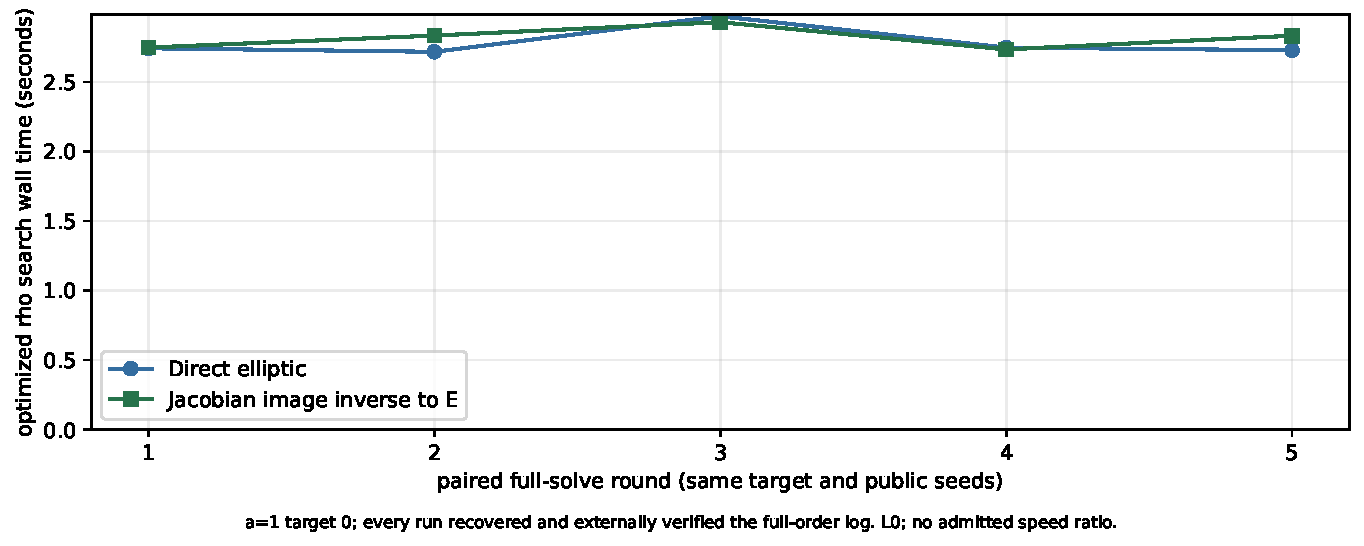
\includegraphics[width=0.98\linewidth]{figures/full-reference-rounds.pdf}\end{center}

The image-inverse arm constructs the two public divisors, checks their inverse,
and runs the same optimized rho on $E_a$. Transfer, setup, search and verification
are recorded separately; the graph shows search only. This establishes a
working full-order transfer-and-solve route. It does not establish an ECDLP
advantage from changing the representation.

\newpage
\textbf{Native Jacobian search.} The separately named resumable method uses
32 lockstep lanes and 32 public jumps, distinguished points, all 166 signed
Frobenius actions, short-cycle escape and a persistent collision table.
All three arms follow the same matched walk. The elliptic arm uses individual
additions; it is distinct from the optimized batched reference on page one.
The Jacobian arm uses checked Cantor addition, then a checked image inverse and
pullback to choose canonical representatives. These conversions and repeated
backend validation are included in its cost. This is a conservative software
implementation, not a benchmark of optimized genus-two formulas or index calculus.

\begin{center}
\begin{tabular}{lrrrr}\toprule
Target & Steps in each arm & E (s) & Inverse/E (s) & Cantor (s)\\\midrule
$Q_0$ & 6,631,641 & 5.846 & 5.842 & 669.526 \\
$Q_1$ & 10,049,968 & 8.937 & 8.726 & 984.515 \\
$Q_2$ & 3,913,125 & 3.392 & 3.423 & 405.053 \\
$Q_3$ & 10,875,029 & 10.603 & 10.859 & 1116.430 \\
\bottomrule\end{tabular}

\end{center}
\IfFileExists{figures/matched-targets.pdf}{
\begin{center}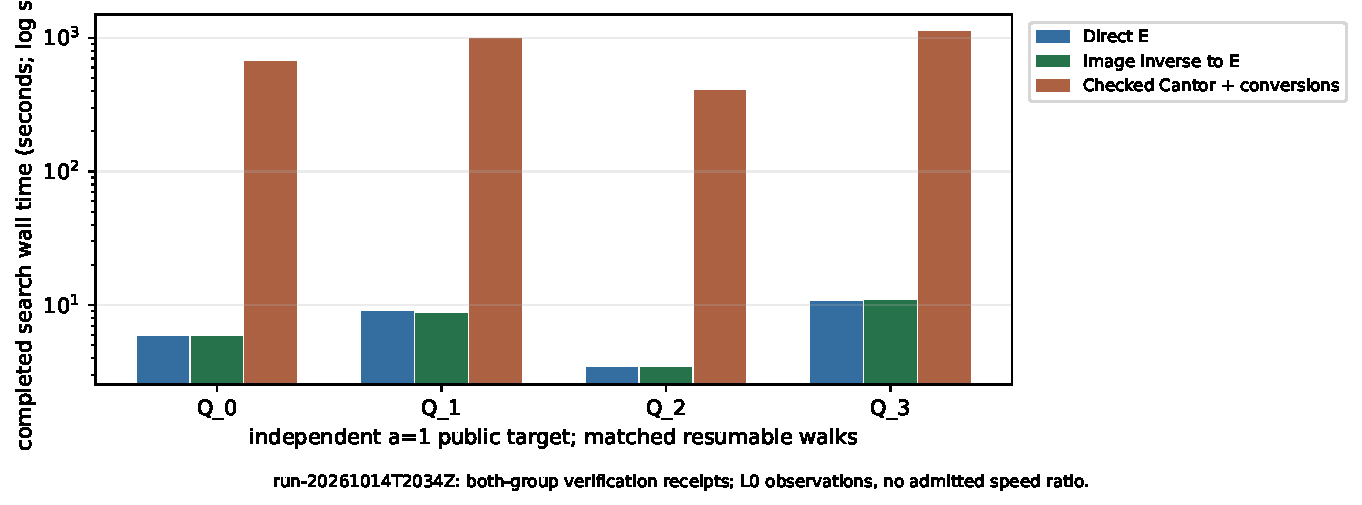
\includegraphics[width=0.98\linewidth]{figures/matched-targets.pdf}\end{center}
}{}

At the acknowledged snapshot, all eight $a=1$ E and inverse/E targets and
seven native Jacobian targets were verified: 23 resumable completions.
Targets $Q_4,Q_5,Q_6$ add three native full solves to the preceding snapshot.
Those three candidates passed a further separate-process check in both groups.
Native $Q_7$ remains unfinished. Earlier verifier receipts are retained.

The $a=0$ checkpoints contain 410,039,272 E steps, 404,195,619 inverse/E
steps and 4,137,664 native Jacobian steps, without candidates. These are
censored work counts, not completed solve times. No target was regenerated.

\newpage
\textbf{Rate calibration.} One warmup, two A/A controls and five interleaved
E/Cantor prefix pairs were recorded per curve. Matching lane digests and
restarted/uninterrupted state checks pass in both repositories. Prefixes are
not completed solves. Counts of E additions and Cantor additions are distinct
native work units; their ratio is not a priced cost ratio.
\begin{center}
\begin{tabular}{rlrr}\toprule
$a$ & Arm & Median steps/s & Observed range\\\midrule
0 & elliptic & 1,051,224 & 911,331--1,101,530 \\
0 & checked Cantor & 10,678 & 10,562--11,008 \\
1 & elliptic & 1,170,906 & 1,153,715--1,175,601 \\
1 & checked Cantor & 11,030 & 10,387--11,158 \\
\bottomrule\end{tabular}

\end{center}
\begin{center}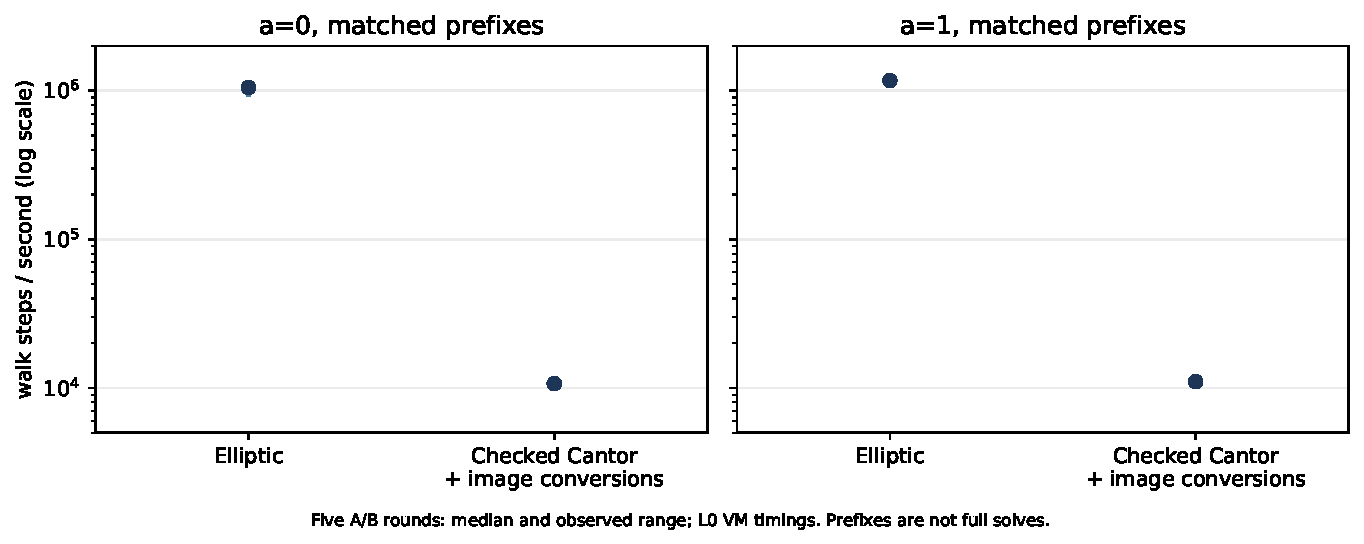
\includegraphics[width=0.82\linewidth]{figures/prefix-rates.pdf}\end{center}

\textbf{Host and admissibility.} Intel Xeon Platinum 8573C virtual worker,
five exposed CPUs, four-CPU quota and 16 GiB memory limit. The native ecbench
primitives take the exclusive benchmark lock, attempt eviction and pin the
solver to CPU 4. Actual affinity is recorded as CPU 4; the observed memory
policy is default. Physical memory type is unavailable. The preflight could
not read CPU/memory PSI, some user threads could not be moved, and hardware
instruction/cycle counters returned \texttt{perf\_event\_open: No such file or directory}.
These are L0 descriptive VM timings. No admitted speedup, common priced-work
ratio, independent-host performance replay or sealed ecbench audit is claimed.
No ARM, GPU or FPGA run was performed.

\textbf{Long campaign and persistence.} The checkpointed worker searches the
complete prime subgroups for both $a$ values. It serially schedules six streams
and advances each arm through eight targets after independent verification.
The $a=1$ native Jacobian stream receives longer quanta to obtain a full native
comparison; $a=0$ work is preserved. Live progress is distinct from frozen
snapshot evidence. Neither an unfinished search nor a birthday-scale rate
projection is a completed solve duration. Current-worker jobs are not durable
against deletion of that worker; the raw checkpoints and exact resume commands
must be retained or moved to another machine.
For $a=0$, the ideal birthday scale divided by the native prefix rate is about
$1.42\times10^7$ seconds on a fully occupied core, before scheduling overhead;
this months-scale heuristic is not a measured duration or calibrated ETA.

Checkpoints include every stored distinguished point, coefficients, lane
histories, cursor and seed/input identity. Writes are atomic and synced. A
pause marker causes a complete snapshot before other heavy work; a stop marker
ends orderly. Reconstruction of native divisor caches is timed as resume work.
Elapsed time determines scheduling only, never a scalar-space restriction.

\newpage
\textbf{Validation and remaining gates.} Both packages pass 33 native unit
tests plus three cover tests, formatting, scoped Clippy, CLI rejection controls
and exact map-identity replay. Identical public-job restart receipts were
obtained in both repositories. The constructed collision unit test is a
correctness control, not a benchmark solve. Backend source remains unchanged;
the preceding whole-library gate still has its two documented JV F4 completion
threshold failures. This report does not call that gate green.

The existing ecbench wide constructor assumes cofactor 4 or 2 and rejects the
$a=1$ pinned prime-factor subgroup. Its counted-group workload has no Mumford
image adapter. The separate native campaign therefore has no ecbench audit
certificate. A registered width-generic adapter, common native-work calibration,
admissible isolation and independent-host replay remain open requirements.
The earlier cover report's geometric Lean bridge also remains partial.

\textbf{Evidence and sources.} Preregistered protocol:
\par{\small\path{research/binary_genus2_speed_20261014/PROTOCOL.md}}\par
Frozen \texttt{runs/run-20261014T2148Z/}, including public jobs, raw per-round/reference
records, verification receipts, host manifests, checkpoint snapshot, source and
binary bindings and SHA-256 manifests. The native summary supplies every plotted
value; the renderer only lays out these recorded values. Both earlier
run snapshots remain unchanged. The 27 optimized reference
runs in the new archive repeat earlier evidence and are not new executions.

Construction proof and identity certificate:
\href{https://github.com/aburan28/crypto/tree/d38a85f7e1ac02358223b58d71633f71f2efa7fa/research/binary_genus2_cover_20261014}{binary genus-two construction study}.
Campaign source and invocation:
\href{https://github.com/aburan28/crypto/tree/dbd33f00da0a0ac35f285603ec168ad9d91a1d79/tools/binary-genus2-cover}{native Rust tool}.
Remaining harness gate: \path{problems/ecbench-binary-genus2-full-subgroup-adapter.md}.
Canonical IC scoreboards and progress graphs were checked for applicability:
this study adds no IC/rho ratio, registered curve or admitted gain, so those
series remain unchanged. The performance visual index receives this report.
\end{document}
